\documentclass[a4paper, 11pt]{article}

\usepackage[utf8]{inputenc}

\usepackage[lmargin=1.5cm,tmargin=2cm,rmargin=1.3cm,bmargin=2cm]{geometry}
\usepackage[onehalfspacing]{setspace}
\usepackage[T1]{fontenc}
\usepackage[brazil]{babel}
\usepackage{float}
\usepackage{polynom}
\usepackage[vlined, portuguese, onelanguage]{algorithm2e}
\usepackage{listings}
\usepackage{xcolor}
\usepackage{titlesec}
\usepackage{verbatim}
\usepackage{circuitikz}
\usepackage{subfigure}

\usepackage{hyperref}
\hypersetup{
    colorlinks = true,
    linkcolor = blue,
    filecolor = magenta,
    urlcolor = cyan,
    citecolor = green,
    pdfpagemode = FullScreen
}

\urlstyle{same}
\usepackage{tikz, pgfplots}
\usetikzlibrary{positioning}

\usepackage{siunitx}
\usepackage[output-decimal-marker={.}]{siunitx}

\usepackage{amsmath,amsthm,amsfonts,amssymb,dsfont,mathtools,blindtext}
\usepackage{cleveref}
\usepackage{graphicx,xcolor,comment,enumerate,multirow,multicol,indentfirst}
\usepackage{graphicx}

\newtheorem{theorem}{Teorema}[section]
\newtheorem{corollary}{Corolário}[theorem]
\newtheorem{definition}{Definição}[section]

\usepackage{stackengine}

\usepackage{lmodern}
%----------------------------------------------------------------------

\pgfplotsset{compat=1.8}

\begin{document}
\section{Binary Logistic Regression}
\begin{center}
        \Large Model
\end{center}

\begin{enumerate}
        \item Binary classification: $y\in\{0,1\}$
        \item Want to predict probability of being in a particular class: $P(y = 1|\mathbf{x};\mathbf{w})$
        \item Could fit a linear model: $f(\mathbf{x};\mathbf{w}) = \mathbf{w}^{T}\mathbf{x}$
        \item But this could give predictions outside $[0,1]$ for some test inputs (invalid probabilities)
        \item Use the sigmoid function to force the output to lie in the $[0,1]$ range:\[f(\mathbf{x};\mathbf{w}) = \frac{1}{1 + e^{-\mathbf{w}^{T}\mathbf{x}}}\]
        \item Interpret $f(\mathbf{x}; \mathbf{w}) = P(y = 1|\mathbf{x};\mathbf{w})$, implying $P(y = 0|\mathbf{x};\mathbf{w}) = 1 - f(\mathbf{x};\mathbf{w})$
\end{enumerate}

\begin{figure}[H]
        \centering
        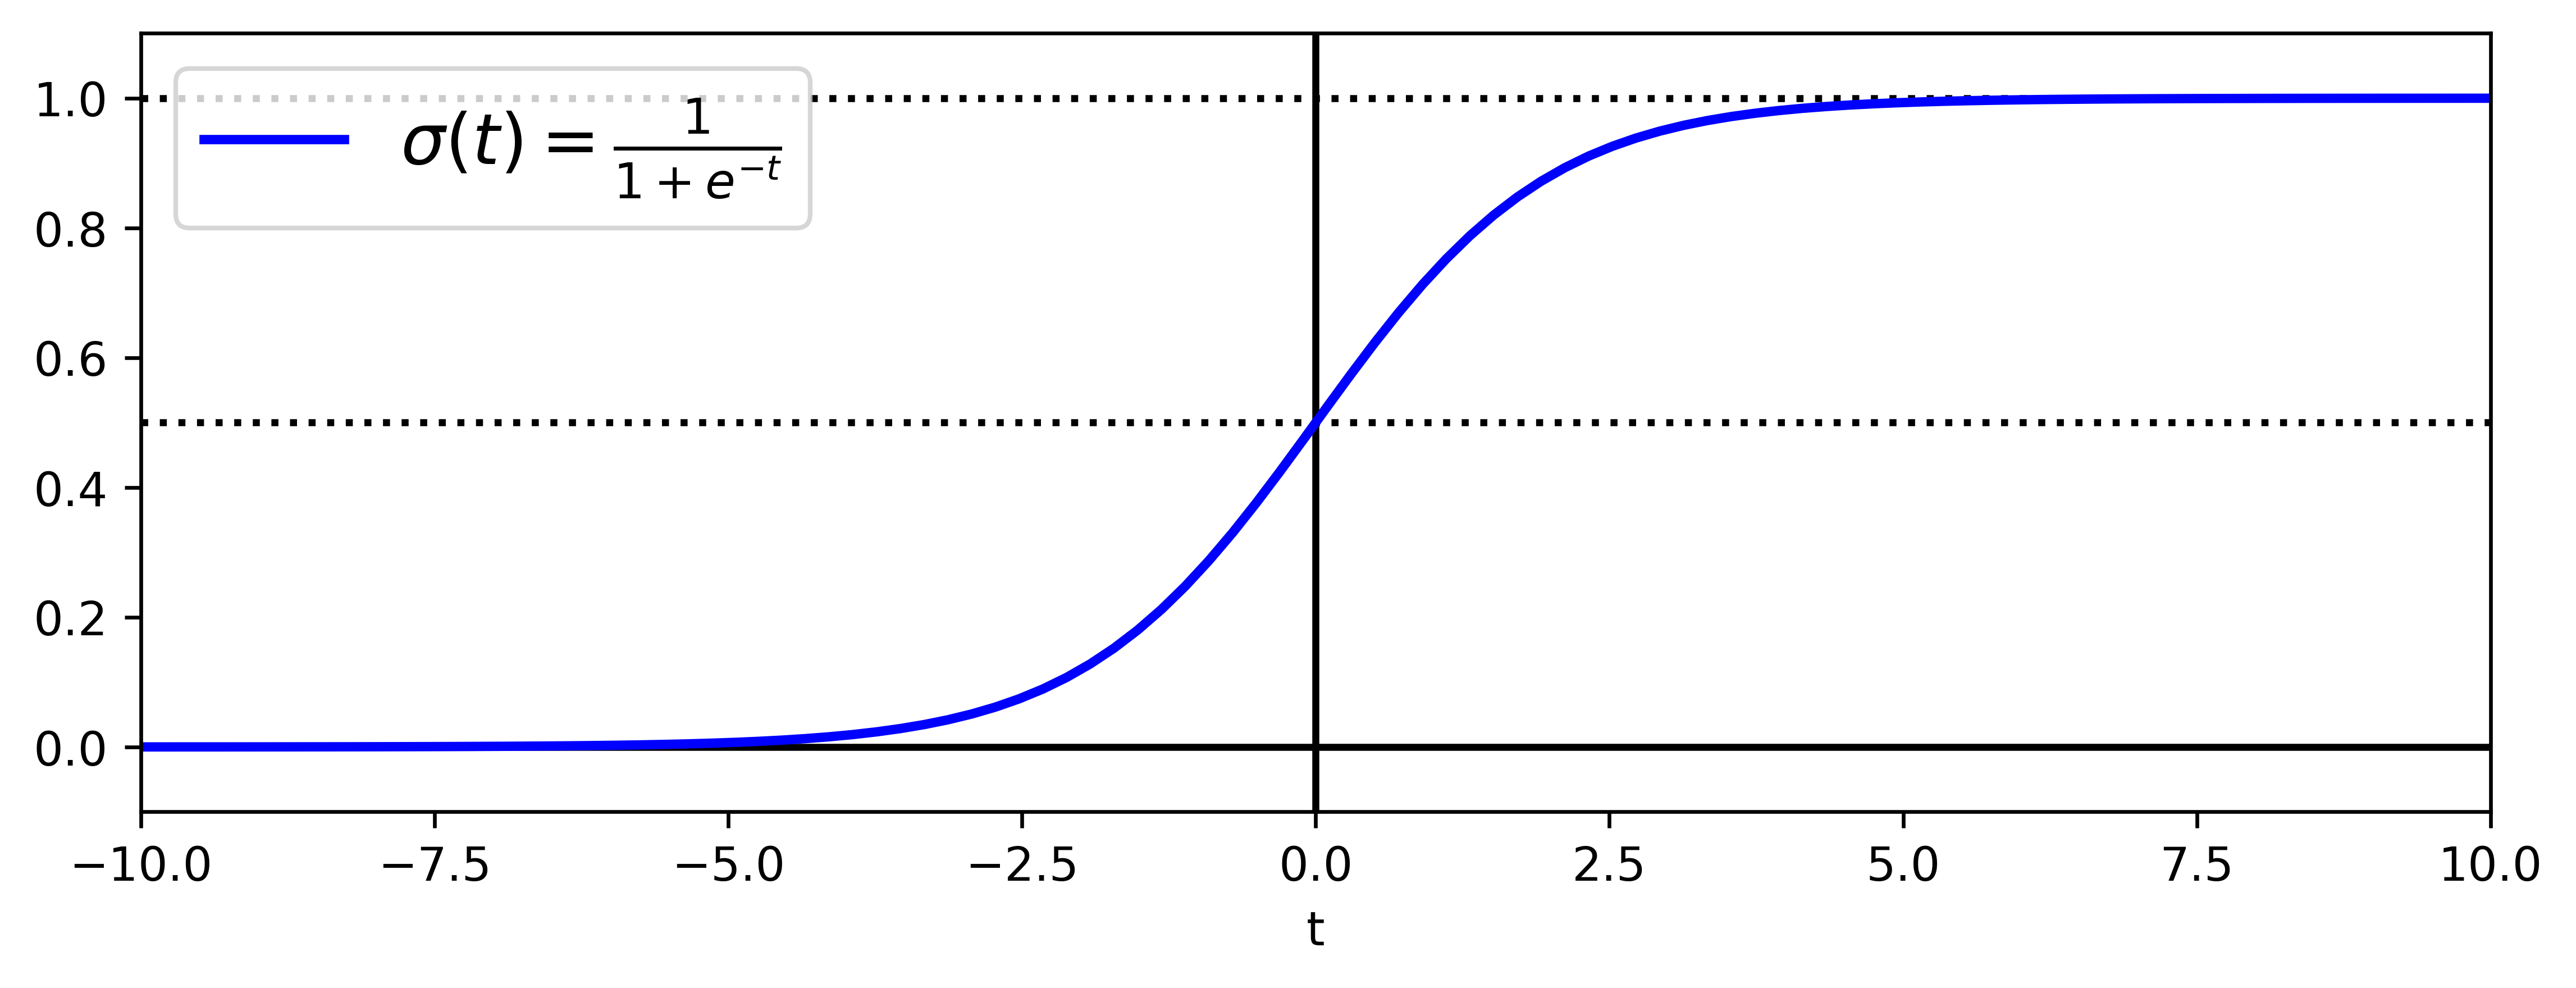
\includegraphics[scale=0.8]{sigmoid.png}
        \caption{Function used to force the output to lie in the $[0,1]$ range}
        \label{fig: Sigmoid Function}
\end{figure}
\newpage
{\Large \textbf{Loss Funciton}}


We observe data $\{(x^{(n)}, y^{(n)})\}_{n = 1}^{N}$, with $y\in\{0, 1\}$, Using maximum likehood:
\begin{align*}
        L(\mathbf{w}) &= P(y^{(1)}|\mathbf{x}^{(1)};\mathbf{w})\cdot P(y^{(2)}|\mathbf{x}^{(2)};\mathbf{w})\cdots P(y^{(n)}|\mathbf{x}^{(n)};\mathbf{w})\\
             &= \prod\limits_{n = 1}^{N}P(y^{(n)}|\mathbf{x}^{(n)};\mathbf{w})
\end{align*}
minimising the negative log likehood
\begin{align*}
        J(\mathbf{w}) &= -\log{L(\mathbf{w})} = -\log{\prod\limits_{n = 1}^{N}P(y^{(n)}|\mathbf{x}^{(n)};\mathbf{w})} = - \sum\limits_{n = 1}^{N}\log{P(y^{(n)}|\mathbf{x}^{(n)};\mathbf{w})}\\
        &(*)\; P(y|\mathbf{x};\mathbf{w}) =\left\{
        \begin{array}{ccc}
                f(\mathbf{x};\mathbf{w}) & if & y = 1\\
                1 - f(\mathbf{x};\mathbf{y}) & if & y = 0
        \end{array}
        \right. = 
        \left\{
        \begin{array}{ccc}
                \sigma(\mathbf{w}^{T};\mathbf{x}) & if & y = 1\\
                1 - \sigma(\mathbf{w}^{T};\mathbf{x}) & if & y = 0
        \end{array}
        \right.\\
        &\implies P(y|\mathbf{x};\mathbf{w}) = \sigma(\mathbf{w}^{T};\mathbf{x})^{y}(1 - \sigma(\mathbf{w}^{T};\mathbf{x}))^{1 - y}\\
        &= -\sum\limits_{n = 1}^{N} \log{[\sigma(\mathbf{w}^{T};\mathbf{x}^{(n)})^{y}(1 - \sigma(\mathbf{w}^{T};\mathbf{x}^{(n)})^{1-y^{(n)}})]}\\
        &= -\sum\limits_{n = 1}^{N} [\log{\sigma(\mathbf{w}^{T};\mathbf{x}^{(n)})^{y}} + (1 - y^{(n)})\cdot\log(1 - \sigma(\mathbf{w}^{T};\mathbf{x}^{(n)}))]
\end{align*}






\end{document}
